% mnras_template.tex
%
% LaTeX template for creating an MNRAS paper
%
% v3.0 released 14 May 2015
% (version numbers match those of mnras.cls)
%
% Copyright (C) Royal Astronomical Society 2015
% Authors:
% Keith T. Smith (Royal Astronomical Society)

% Change log
%
% v3.0 May 2015
%    Renamed to match the new package name
%    Version number matches mnras.cls
%    A few minor tweaks to wording
% v1.0 September 2013
%    Beta testing only - never publicly released
%    First version: a simple (ish) template for creating an MNRAS paper

%%%%%%%%%%%%%%%%%%%%%%%%%%%%%%%%%%%%%%%%%%%%%%%%%%
% Basic setup. Most papers should leave these options alone.
\documentclass[fleqn,usenatbib]{mnras}  % a4paper,

% MNRAS is set in Times font. If you don't have this installed (most LaTeX
% installations will be fine) or prefer the old Computer Modern fonts, comment
% out the following line
\usepackage{newtxtext,newtxmath}
%\usepackage{txfonts}
% Depending on your LaTeX fonts installation, you might get better results with one of these:
%\usepackage{mathptmx}
%\usepackage{txfonts}


\usepackage[export]{adjustbox}

% Use vector fonts, so it zooms properly in on-screen viewing software
% Don't change these lines unless you know what you are doing
\usepackage[T1]{fontenc}
\usepackage{ae,aecompl}
%\usepackage{slashbox}


\usepackage{natbib}


%%%%% AUTHORS - PLACE YOUR OWN PACKAGES HERE %%%%%

% Only include extra packages if you really need them. Common packages are:
\usepackage{graphicx}	% Including figure files
\usepackage{amsmath}	% Advanced maths commands
\usepackage{amssymb}	% Extra maths symbols
\usepackage{diagbox}
%%%%%%%%%%%%%%%%%%%%%%%%%%%%%%%%%%%%%%%%%%%%%%%%%%

%%%%% AUTHORS - PLACE YOUR OWN COMMANDS HERE %%%%%

% Please keep new commands to a minimum, and use \newcommand not \def to avoid
% overwriting existing commands. Example:
%\newcommand{\pcm}{\,cm$^{-2}$}	% per cm-squared

%%%%%%%%%%%%%%%%%%%%%%%%%%%%%%%%%%%%%%%%%%%%%%%%%%

%%%%%%%%%%%%%%%%%%% TITLE PAGE %%%%%%%%%%%%%%%%%%%

% Title of the paper, and the short title which is used in the headers.
% Keep the title short and informative.
\title[Quasar Variability]{Solving the puzzle of discrepant variability on monthly time scales implied by SDSS and CRTS datasets}

% The list of authors, and the short list which is used in the headers.
% If you need two or more lines of authors, add an extra line using \newauthor
\author[K. Suberlak et al.]{
Krzysztof Suberlak,$^{1}$\thanks{E-mail: suberlak@uw.edu}
\v{Z}eljko Ivezi\'c, $^{1}$
Chelsea L. MacLeod,$^{2}$
Matthew Graham,$^{3}$ 
\newauthor
$\, \,  $Branimir Sesar$^{4}$
\\
% List of institutions
$^{1}$Department of Astronomy, University of Washington, Seattle, WA, United States\\
$^{2}$Institute for Astronomy, University of Edinburgh, Royal Observatory, Edinburgh, United Kingdom\\
$^{3}$Center for Data-Driven Discovery, California Institute of Technology, Pasadena, CA, United States\\
$^{4}$National Optical Astronomy Observatory, Tucson, AZ, United States.
}

% These dates will be filled out by the publisher
\date{Accepted XXX. Received YYY; in original form ZZZ}

% Enter the current year, for the copyright statements etc.
\pubyear{2016}

% Don't change these lines
\begin{document}
\label{firstpage}
\pagerange{\pageref{firstpage}--\pageref{lastpage}}
\maketitle

% Abstract of the paper
\begin{abstract}

We present improved error analysis for the 7,100 CRTS (Catalina Real-Time Transient Survey) optical  light curves for quasars from the Sloan Digital Sky Survey Stripe 82 catalog. SDSS imaging survey has provided a time-resolved photometric  dataset which greatly improved our understanding of the quasar optical continuum variability: data for monthly and longer timescales  are consistent with a damped random walk. Recently, newer data  obtained by CRTS provided  puzzling evidence for enhanced variability, compared to SDSS results, on monthly time scales. Quantitatively, SDSS results predict  about 0.06 mag root-mean-square variability for timescales below 50 days, while CRTS data show about a factor of two larger rms for spectroscopically confirmed SDSS quasars. Our analysis presented here has successfully resolved this discrepancy as due to slightly underestimated photometric uncertainties provided by the CRTS image processing pipelines. The photometric error correction factors, derived from detailed analysis of non-variable SDSS standard stars that were re-observed by CRTS, are about 20-30\%, and result in a quasar variability behavior implied by the CRTS data that is fully consistent with earlier SDSS results.


\end{abstract}


%%%%%%%%%%%%%%%%%%%%%%%%%%%%%%%%%%%%%%%%%%%%%%%%%%

%%%%%%%%%%%%%%%%% BODY OF PAPER %%%%%%%%%%%%%%%%%%

\section{Introduction}
Variability can be used to both characterize and select quasars  in sky surveys (for a recent overview, see \cite{lawrence2016a}) . Although various time scales of variability can be linked to physical parameters, such as accretion disk viscosity, or corona geometry (\cite{kelly2011}, Graham+2014), the physical mechanism remains elusive, and most viable explanations include accretion disk instabilities  \citep{kawaguchi1998}, surface thermal fluctuations from magnetic field turbulence \citep{kelly2009}, coronal x-ray heating \citep{kelly2011} (see \cite{kozlowski2016} for review).
The diversity of  physical scenarios available to explain the origin of quasar variability results in a variety of ways to characterize it. The two most widely used approaches to describe variability of quasars  are damped random walk (DRW) and structure function (SF). The DRW model is more suited for light curves with a typical cadence of days \citep{zu2013, kozlowski2016}, whereas an ensemble SF analysis is better for sparsely sampled light curves \citep{hawkins2002, berk2004,   devries2005, schmidt2010, graham2014}, or review in \cite{kozlowski2016}). For CRTS sparsely sampled light curves we prefer the SF approach, as more robust  than fitting for DRW parameters.

Although SF can be defined  in a variety of ways, it can be characterized by a simple broken power law \citep{schmidt2010}. At short timescales,  the variability amplitude increases, following a steeper power law index,  until the power law index starts to flatten  above the characteristic timescale  $\tau$.   This knee in the power law  description may correspond to a transition from the stochastic thermal  process driving  the variability, to the physical response of the disk that successfully  dampens the amplitude on longer timescales (\cite{lawrence2016a, kelly2007,kelly2009, kelly2011, peterson2001} ,  (linking the amplitude to the black hole mass)). Indeed,  in x-rays quasars are described by a broken  power law, where the  break timescale is linked to the size of x-ray emitting region ( \cite{kelly2011} in \cite{graham2014}). 

Altough previous studies found that  $\tau > 100$ days  (\cite{macleod2010},  \cite{kozlowski2016}), recently, \cite{graham2014} used the SF, DRW, and Slepian Wavelet Variance (SWV) analysis for CRTS and SDSS S82 lightcurves. Using SWV on CRTS data they found characteristic time scales at   QSO rest frame of $\log_{2}(\tau) = 5.75$)  54 days,  and ($\log_{2}(\tau)=8.2$) -  294 days. Additionally, using this method on S82 data they found a peak at $\log_{2}(\tau) = 7.25$ , and for OGLE  at $\log_{2}(\tau)$ $> 6$ . The short timescale of   $\tau = 54$ days is surprising, as it is shorter by a factor of two than any previous estimates \citep{macleod2011, zu2013}. We set out to reanalyze the CRTS data, and investigate the plausibility of these discrepant timescales. 


\section{Data Sets}

We study stars and quasars from  Stripe 82 (S82), using the  Sloan Digital Sky Survey   and the Catalina Real-time Transient Survey data. S82 is a large (over 100 deg$^{2}$), repeatedly observed reqion of the equatorial sky ($22^{h} 24^{m} < \mathrm{RA} < 04^{h} 08^{m}$ and $\mathrm{| Dec |} < 1.27 deg$)    \citep{sesar2007, suveges2012}. 	

\subsection{Sloan Digital Sky Survey (SDSS)}
We use the SDSS catalog data with  robust,  five-band near-simultaneous  photometry for  9258  quasars,  and 1006849 standard stars - we use it for photometric color information and sample selection.  The  quasar catalog \footnote{\url{http://www.astro.washington.edu/users/ivezic/cmacleod/qso_dr7/Southern.html}} contains spectroscopically confirmed quasars from the SDSS Data Release 7 \citep{abazajian2009}, based on the SDSS Quasar  Catalog IV (\cite{schneider2008} VizieR Online Data Catalog, 7252, 0), and was compiled by \cite{macleod2011} . The standard stars catalog\footnote{\url{http://www.astro.washington.edu/users/ivezic/sdss/catalogs/stripe82.html}} ver. 2.6 was compiled by \cite{ivezic2007}.

\subsection{Catalina Real-time Transient Survey (CRTS)}
The CRTS data consists of white light (no filter) lightcurves  - it was designed to find near-Earth objects, hence short intra-night cadence, to allow a rapid follow up \citep{graham2015b} .  Three survey telescopes (0.7m Catalina Sky Survey Schmidt in Arizona,  1.5m Mount  Lemmon Survey telescope in Arizona, and the 0.5m Siding Spring Survey Schmidt in Australia) were equipped with identical, 4kx4k CCDs taking 4 exposures each night (see \cite{djorgovski2011a} for technical details).
Although in principle white light magnitudes can be calibrated to Johnson V-band zero point \citep{drake2013}, we found this step redundant in our analysis. 

In this study we used a sample of 7932 spectroscopically confirmed S82  quasars,   prepared by B. Sesar, from  the Data Release 2, based on the list by \cite{macleod2011}.  The majority (96\%) of  CRTS quasar lightcurves span the time of 7-9 years, with a mean sampling of 1 to 4 times per night,  on 70 nights on average (see Fig.1, upper-left panel).  Mean interval between epochs is 209 days (\ref{fig:1} bottom-right panel), and the mean quasar magnitude is 19.5 mag. 

For comparison we use the CRTS lightcurves of 52133 randomly chosen  10\% of the S82 standard stars catalog ver.2.6 \citep{ivezic2007}, extracted by B. Sesar from the CRTS Data Release 2.

\begin{figure}
\label{fig:1}
 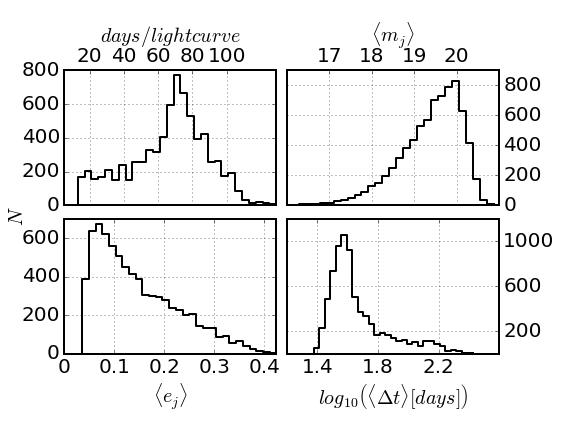
\includegraphics[width=\columnwidth]{Fig_1_QSO_CRTS_proc_stats.png}
 \caption{The properties of 7601 day-averaged CRTS quasar lightcurves that have over 10 day-averaged epochs. The upper-left panel shows the distribution of the lightcurve length after day averaging, corresponding to the number of distinct days on which CRTS quasars were observed. The mean of quantities on the following three panels corresponds to the average over a lightcurve. First, the upper-right panel shows the mean day-averaged CRTS magnitude, $\langle  m_{j} \rangle$ (see eq.~\ref{eq:1}). Second, the bottom-left panel shows the  mean day-averaged lightcurve error, $\langle \sigma_{j} \rangle$ (see eq.~\ref{eq:2}). Finally, the bottom-right panel depicts the average time  difference between day-averaged epochs,  $\langle \Delta t \rangle$. Within that sample , $96 \% $ observations of quasars span the time of 7-9 years.  $91.2\%$ of  quasars were observed between 1 to 4 times per night. We use only quasars with light curve averaged error smaller than 0.3, leaving 7108 quasars in the sample.}
\end{figure}



\subsection{Catalog Matching}
To enrich the information about each CRTS object with SDSS color information, we matched positionally the CRTS data to the SDSS data within the S82 using astropy \citep{robitaille2013} \verb|match_to_catalog_sky|  routine\footnote{\url{http://docs.astropy.org/en/stable/coordinates/matchsep.html\#matching-catalogs}}.  
Since the SDSS catalog has over 10 times more stars than CRTS, we found an SDSS counterpart to all  CRTS stars within 0.01 arcsec matching radius. The SDSS S82 quasar catalog is not significantly larger than CRTS catalog, and for 7586 CRTS quasars we found an SDSS counterpart within 0.36 arcsec.   We  ignored  15 CRTS quasars for which no SDSS counterpart was found within 1 arcsec.  


\subsection{Preprocessing}

It is common to bin the data to reduce noise, by averaging over timescales shorter than what is required by the science goals. In this study, the hourly timescale of intra-night variability of CRTS lightcurves, with $\approx 4$ epochs each night, is much shorter than the timescales of interest on the order of tens of days.  Thus, as part of preprocessing we day-averaged all  CRTS light curves, following a procedure similar to \cite{charisi2016}. We adopt a convention that an index  $i$ runs over intra-night observations, and an index $j$ separates distinct observing nights. Thus the day-averaged timestamp is : 
\begin{equation}
t_{j} = \langle t_{ij} \rangle = \frac{\sum_{i=1}^{N}{ t_{ij} }} {N} 
\end{equation}
where $i=1...N$, is the number of observations per night. We similarly replace each set of N brightness measurements from the  $j$-th  night by their mean weighted by the inverse square of error:
\begin{equation}
\label{eq:1}
 m_{j} = \langle m_{ij} \rangle = \frac{\sum_{i=1}^{N} {w_{i,j} m_{i,j}} } {\sum_{i=1}^{N} {w_{i,j}} }
\end{equation}
with weights $w_{i,j} = e_{i,j}^{-2}$.  

Finally, we estimate the error on the weighted mean $m_{j}$ by the inverse square of the sum of weights:  
\begin{equation}
\label{eq:2}
\sigma_{j}(m_{j}) = \frac{1}{\sqrt{\sum_{i}{w_{i,j}}}}
\end{equation} and to avoid unphysically small errors, we add in quadrature 0.01\textsuperscript{mag}  to $\sigma_{j}$ if $\sigma_{j} < 0.02$\textsuperscript{mag}. 


\subsection{Selection}
We have selected both quasars and stars using a combination of information from SDSS and CRTS. To find magnitude difference between different days we first require that the raw lightcurve has more than 10 epochs, which from initial 52131 stars and 7932 quasars left 49385 stars and 7707 quasars. We thus also remove those lightcurves with less than 10 days of observations, leaving 7601 quasars and 48250 stars.  We also require that the lightcurve-average of day-error $\langle \sigma_{j}(m_{j}) \rangle < 0.3$\textsuperscript{mag} (see Fig.\ref{fig:1}). Since the raw distribution of errors peaks at lower values (mean of 0.19\textsuperscript{mag} for stars and 0.22\textsuperscript{mag} for quasars) than the distribution of the weighted mean errors (mean of 0.13\textsuperscript{mag} for stars and 0.15\textsuperscript{mag} for quasars), this cut only removes less than 10\% of lightcurves. Our final sample consists of 7108 quasars and 42864 stars.

\section{Analysis Methods}
\label{sec:analysis}
% opening sentence
To analyze the quasar and stellar lightcurves we consider a relationship between measured data $m_{j}$  at times $t_{j}$, and its "copy" shifted by $\Delta  t$ \citep{kozlowski2016}. We simultaneously consider all differential points for a given object type, binning the magnitude differences according to the time shift  $\Delta t$.  For each bin we calculate  statistical properties that characterize the variability. By comparing quasars to stars split by color into "blue" and "red" groups, we infer that from CRTS data their variability is consistent with noise at short timescales ($\log_{10}\Delta t < 1.7 $) . 

\subsection{Structure Function}
% What is SF
The structure function is a well-studied approach to characterizing lightcurves \citep{berk2004, devries2005, kozlowski2016, graham2013} . To avoid the uncertain redshift estimate from the SDSS spectra that would be required to correct to the rest-frame variability, for the majority of analysis we use the observed frame time lags (see \cite{schmidt2010, kozlowski2016}).   Thus, for two day-averaged epochs $j$ and $k$, $j > k$ the  magnitude difference is $\Delta m_{j,k} = m_{j} - m_{k}$, the time difference is  $\Delta t_{j,k} = t_{j} - t_{k}$, and the combined error is $\sigma_{j,k}^{2} = \sigma_{j}^{2} + \sigma_{k}^{2}$. 
%[NOTE : Graham+2014 uses observed and rest-frame interchangeably - some timescales are quoted in %observed, the others in restframe... ]

% Binning
To study the statistical distribution of ensemble time-lag magnitude differences we bin the data along $\Delta t_{j,k} $, or for brevity  $\Delta t$ (similar convention for $\Delta m$ and $\sigma$). For each object  we prepared 'master' files containing $\Delta m$, $\Delta t$, $\sigma$. Each object, with a median lightcurve length of 70 days,  contributes on average $\sum_{j=2}^{70}{(j-1)} = 2415$  $\Delta m$ points . Thus we have sufficient amount of $\Delta t$ points to study their statistical properties by splitting them into 200 linearly spaced bins of  $\Delta t$. Bin number does not affect significantly the shape of the structure function, and 200 bins is a good choice to provide adequate time resolution and ensure a large number of  $\Delta m$ in each bin.

% Structure Function 
With  various theoretical definitions of structure function (see \cite{kozlowski2016} for overview), we adopt a view from \cite{ivezic2014}, that $SF$ corresponds to the intrinsic width of the $\Delta m$ distribution  $\mathcal{N}(\sigma,\mu)$. Consider all N  $\Delta m$  points in a certain $\Delta t$  bin.  Each point has an error, which we assume is drawn from the Gaussian distribution with a known width $e_{i}$ (here index $i$ runs over all points in a given $\Delta t$ bin). Thus each $\Delta m$ (called $x_{i}$ for brevity, as  in  \cite{ivezic2014}), is drawn from a distribution  with a total width $\sigma_{tot} = \sqrt{\sigma^{2} + e_{i}^{2}}$. 

Then the likelihood for a set of measurements $\{x_{i}\}$ is given by a product of likelihoods for each value of $x_{i}$:

\begin{equation}
p(\{ x_{i}\} | \mu, \sigma, I) =  \prod _{i=1}^{N} { \frac{1}{\sqrt{2\pi \sigma_{tot}}} \exp{\left( \frac{-(x_{i}-\mu)^{2}}{2\sigma_{tot}^{2}} \right)}}
\end{equation}

Using uniform priors, the logarithm of the posterior pdf is :

\begin{equation}
\label{eq:logP}
L_{p} = const - \frac{1}{2} \sum_{i=1}^{N} {\left( \ln{(\sigma_{tot}^{2})} + \frac{(x_{i}-\mu)^{2}}{\sigma_{tot}} \right) }
\end{equation}

To find $SF = (\sigma)$, we evaluate $L_{p}$ on a grid of $\mu, \sigma$, and marginalize over $\mu$ to find likelihood for $\sigma$:  

\begin{equation}
p(\sigma|\{ x_{i}\}, I) = \int_{0}^{\infty} {p(\mu,\sigma |\{ x_{i}\}, I )} d \mu
\end{equation}

The zero point of the first derivative of this likelihood: $\sigma_{0}$,  is the most likely value of $\sigma$. An alternative way is to find the $2D$ maximum of $\exp{(L_{p})}$ to obtain simultaneously both $\mu_{0}$ and $\sigma_{0}$. However, without any prior constraint on the value of $\mu_{0}$ or $\sigma_{0}$ this procedure can be  computationally expensive. Thus we first find  approximate values of  $\sigma_{0}$ and $\mu_{0}$.  The sample median is a good estimator of $\mu_{0}$, and $\sigma_{0}$ can be estimated by:

\begin{equation}
\sigma_{0}^{2} = \zeta^{2} \sigma_{G}^{2} - e_{50}^{2}
\end{equation} 
where:
\begin{equation}
\zeta = median(\tilde{\sigma_{i}}) / mean(\tilde{\sigma_{i}}),
\end{equation} 
\begin{equation}
\tilde{\sigma_{i}} = (\sigma_{G}^{2} + e_{i}^{2} - e_{50}^{2})^{1/2},
\end{equation}
\begin{equation}
\sigma_{G} = 0.741 (Z_{75\%} - Z_{25\%}), 
\end{equation}
where $Z$ is the sorted $\Delta m$ per bin, and $e_{50} = median(\sigma)$.

Now, if errors were all equal ($e_{i} = e$), then $e_{50} = e$, and $\tilde{\sigma_{i}}= \sigma_{G}$, so that $\zeta=1$ , and thus $\sigma_{0}^{2} = \sigma_{G}^{2} - e^{2}$. 

If errors were not all equal, but very small compared to $\sigma_{G}$, then $\tilde{\sigma_{i}} \to \sigma_{G}$, and $\zeta \to 1$, so that  $\sigma_{0}^{2} = \sigma_{G}^{2} - e_{50}^{2}$, but since $e_{50} \ll \sigma_{G}$,  $\sigma_{0}^{2} \approx \sigma_{G}^{2}$. This explains why $\sigma_{G}$ can be seen as an approximation of $SF$ (see eq.10 in \cite{kozlowski2016}). 

Therefore, to find the best estimate of $SF = \sigma_{0}$, we evaluate 1000 boostrapped resamples of $\Delta m$ in each $\Delta t$ bin, and hence find upper and lower limits on the approximate value of $\sigma_{0}$. We use these values as limits on our grid  of  $\mu$, $\sigma$, on which we evaluate the full solution from  $L_{p}$. 


\subsection{Statistics, sample construction}
\label{sec:stats}
% What is on the four-panel plot: SF, st dev , sigmaG, mu  
As described above, $\sigma_{0}$, $\sigma_{G}$ and $\mu$ are all related in describing the structure function and variability of quasars, and thus we plot them as a function of $\Delta t$ on Fig.~\ref{fig:2}. As a guide to the width of the $\Delta m$ distribution, we also plot its standard deviation, i.e. the square root of the average of the squared deviations from the mean:
\begin{equation}
\sigma_{stdev} = \sqrt{ \frac{\sum\left(\Delta m - \overline{\Delta m}\right)^{2} } { N_{bin}}}   
\end{equation}

% color selection
To consider the effect of stellar color on variability we divided the sample of stars into two SDSS g-i color bins: "red" stars with $1<g-i<3$, and  "blue" stars with $-1<g-i<1$. We expect blue stars to be preferentially brighter, and have smaller variability than the red stars. See Table ~\ref{tab:object_count} for the number of stars and quasars in each color-magnitude bin. 

\begin{table}
\centering
\caption{Count of stars and quasars, selected by their SDSS r-magnitude. For all objects we also required that the CRTS lightcurve error is smaller than $0.3$ mag.}
\label{tab:object_count}
\begin{tabular}{ l|ccc } 
% \hline
r-mag  & red stars & blue stars & quasars \\ 
 \hline
17-18   & 2993 & 2795   & 185    \\ 
18-18.5 & 2087 &  1400  & 333   \\ 
18.5-19 & 1496 &  2327  & 747   
% \hline
\end{tabular}
\end{table}
 
% magnitude selection  
To consider any magnitude-dependent trends in the data, such as increasing photometric error for fainter objects, we split our sample into three magnitude bins: bright  17-18,  medium 18-18.5 , and faint  18.5-19\textsuperscript{mag}. We used SDSS r-magnitude to select the magnitude of objects, which is correlated to the CRTS white light magnitude for both stars and quasars. Table~\ref{tab:object_count} shows the number of objects per magnitude bin.  

\begin{figure}
\label{fig:2}
 \includegraphics[width=1.2\columnwidth, center]{{Fig_2_18.5-19_panels}.png}
 \caption{The four panels show statistics calculated for the subsample of 333 CRTS quasars (black points), 1400 "blue" stars (blue points), and 2087 "red" stars (red points), all  chosen according to the SDSS r magnitude $18.5 < \mathrm{m} < 19$. Red and blue stars have  $1 < \mathrm{g-i} < 3$ and  $-1 < \mathrm{g-i} < 1$ respectively. All pairwise brightness differences  in white light ($\Delta m_{i,j}$) are binned in 200 linearly spaced bins of $\Delta t_{i,j}$. For each bin, we calculate different statistics, from top to bottom panels: the standard deviation $\sigma_{stdev}$, the robust Gaussian deviation based on the interquartile range $\sigma_{G}$, the structure function $SF$, and  the mean value of $\Delta m_{i,j}$  per bin:$\mu$. Both $\mu$ and $\sigma$ are found from the 2D maximum of the log-likelihood $L_{p}$ on the $[\mu,\sigma]$ grid (see eq.~\ref{eq:logP}, and \citep{ivezic2014}).  Yellow dashed line on the third panel traces the fiducial Damped Random Walk model. Note how the level of variability for both blue and red stars does not increase with timescale (staying on ~0.1 mag level), unlike quasars. Since the variability of stars corresponds here to the measurement noise, until quasars raise above the stellar structure function level (at  $\log{ \Delta t} > 2$), no claim can be made about their intrinsic variability.   Thus any departure of CRTS quasar structure function at low timescales ($\log{\Delta t} < 1.7$ ),   is due to incorrect errors (underestimated measurement noise).}
 % The signal modulation  - wiggles - also seen when we simply plot the number 
 % of points per bin as a function of log(delta t) .  
 % Not due to number of points  - the scatter of some distribution does not depend 
 % on sample size (email from 	12/06/16 )
\end{figure}


\section{Results}
\label{sec:results}
% "what we measured"
% "how it affects other theories"
% "further tests / theories to challenge?"   
% "patiently teach, and walk before you run" 


%the problem : Fig 2 
The measured level of variability for standard stars is above the acceptable 0.05\textsuperscript{mag} rms, and is incompatible with their known non-variability. Fig.2 illustrates the problem, using the four statistics calculated for the 18.5-19\textsuperscript{mag} bin, as described in Sec.~\ref{sec:stats}.  Especially $SF$ shows that even on short timescales, stars exhibit a non-zero variability for stars. Based on the SDSS data concerning the same stars, we would expect their SF to be below the level of noise : 0.05\textsuperscript{mag} \citep{ivezic2007}. This larger than expected variability is inspected in more detail in Fig.\ref{fig:3}. 


%finding the solution : Fig 3 
  %- description of what we are plotting 
We derive correction factors for CRTS photometric errors using blue stars, since they  have similar colors to quasars. Consider the robust with of $\chi$ distribution:

\begin{equation}
\chi_{i} = \frac{\Delta m_{i} - \overline{\Delta m_{i}}}{\sigma_{i}}
\end{equation}

for pairwise magnitude difference points, but since our lightcurves are symmetric around 0, $\overline{\Delta m_{i}} \approx 0$.  It is worth noting that $\chi_{i}$ is related to chi-square: 

\begin{equation}
\chi^{2} = \sum_{i=1}^{N}{\chi_{i}^{2}}
\end{equation}

Therefore, if $\sigma_{i}$ describes well the underlying (Gaussian) error, then in case of no intrinsic variability we would expect $\sigma_{G}(\chi) = 1$,  such as is the case for blue standard stars. 

We binned the time lag - magnitude difference points into four $\log (\Delta t ) $ bins : one for short timescales  $\log \Delta t < 1.7$ ($\Delta t < 50$ days), and three for longer timescales : $\log \Delta t \in (2.3,2.5)$, $\log \Delta t \in (2.8,3.0)$, and $\log \Delta t \in (3.2,3.4)$.  We also split the sample in three magnitude bins, which together results in 12 separate $\log\Delta t$ - magnitude bins for blue stars and quasars. This allows to check whether there is any dependence of error correction on magnitude or timescale.  For each bin we evaluate the histogram of a quantity $\chi$. As shown on Fig.\ref{fig:3}, the width of $\chi$ distribution differs from 1 for blue stars, which means that $\sigma_{i}$ is either over or under-estimated. Furthermore, at short timescales ($\log{\Delta t} < 1.7$) quasars are indistinguishable from stars in $\chi$. However, at longer timescales quasars show distinct signature of variability - the distribution of $\chi$ is much wider for quasars than for stars. To correct the discrepant robust width of stellar $\chi$, we find the correction factor based on the $\sigma_{G}(\chi_{blue})$.  We find that for blue stars there is a magnitude-dependent  linear relationship between the robust width of $\chi$ distribution, and the $\log{\Delta t}$, but the $\log{\Delta t}$ dependence is an order of magnitude smaller than the magnitude dependence. Therefore we average the value of  $\sigma_{G}(\chi_{blue})$   over all timescales for each magnitude bin, resulting in a single value of correction factor, $f_{c}$, per magnitude bin (see Table~\ref{tab:fc}).  

% For each magnitude bin we fit a straight line, and thus find linear correction coefficients, according to 
%\begin{equation}
%\label{eq:fc}
%f_{c} = \sigma_{G}(\chi_{Blue}) = a  \, \log_{10}(\Delta t) + b
%\end{equation}
%(see Table 2). We find that higher order polynomial unnecessary, given that the standard deviation of straight line fit is smaller than  0.003, i.e. less than $1\%$ level. 

Multiplying  $\sigma_{i}$ by the corresponding f\textsubscript{c} brings  $\sigma_{G}(\chi_{Blue})$ to 1, as expected. We thus correct the day-averaged errors, which brings down the variability (see Fig.~\ref{fig:4}):

\begin{equation}
\sigma_{i,corr}  = f_{c} \, \sigma_{i}  
\end{equation} 

As we show in Appendix A, it also is a multiplicative constant that can be applied to correct the raw photometric errors: 

\begin{equation}
e_{corr} = f_{c} \, e
\end{equation}

\begin{table}
\centering
\caption{The correction coefficients, as evaluated from  $\sigma_{G}(\chi)$ for blue stars.}
\label{tab:fc}
\begin{tabular}{ l|cc } 
% \hline
correction & mag \\ 
 \hline
0.0870 &  17   - 18  \\
1.1072  &  18   - 18.5  \\
1.2876  &  18.5 - 19  
% \hline
\end{tabular}
\end{table}


\begin{figure}
\label{fig:3}
%\centerfloat
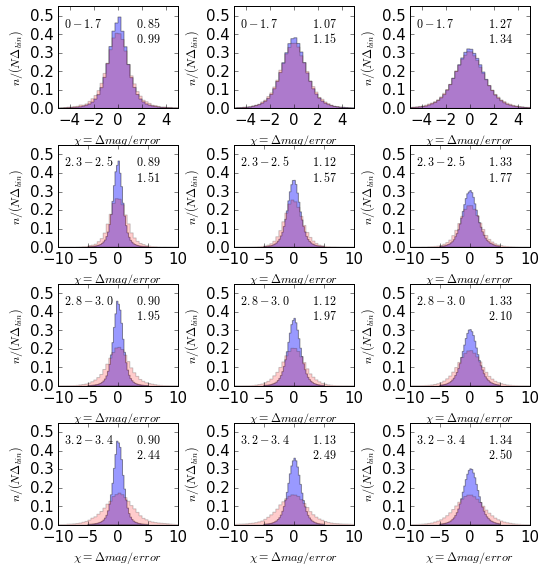
\includegraphics[width=1.15\columnwidth, center]{Fig_3_histogram_panels.png}
 \caption{This grid of histograms shows $\chi = \Delta m / \mathrm{error}$ for CRTS blue stars (blue shading) and quasars (red shading), split into bins of $\log{\Delta t}$- SDSS r magnitude. Vertically, from top to bottom, we iterate over bins of $\log{\Delta t}$ : $0<\log{\Delta t}<1.7$ ($t < 50 $ days), $2.3<\log{\Delta t}<2.5$, $2.8<\log{\Delta t}<3.0$, and $3.2<\log{\Delta t}<3.4$ (indicated by numbers in the upper left corner of each subplot). Horizontally, from left to right, we iterate over SDSS r-magnitude bins $17-18$,  $18-18.5$, and $18.5-19$. Objects in each vertical strip were chosen according to the same magnitude cut, and all $\Delta m$ points in a given  $\log{\Delta t}$ range were binned together. The  implied small quasar variability at short timescales is at the level  measured by SDSS (indistinguishable from blue, non-variable stars). Numbers in the upper-right corner of each subplot are the robust width of stellar  and quasar  distributions of $\chi$. Blue, bright  stars in the left strip (17-18\textsuperscript{mag}) have low $\sigma_{G}$, at the level of 0.9, and fainter blue stars (eg. right vertical strip, 18.5-19\textsuperscript{mag}) have higher $\sigma_{G} \approx 1.3$. Part of that increase is due to larger errors at fainter magnitude end. However, in each bin we expect that if errors for blue stars are correct, then  $\sigma_{G}(\chi) = 1$. We use  correction factors $f_{c} = \sigma_{G}(\chi_{blue}(\Delta t, mag))$ to correct for that effect. This implies that magnitude-difference errors  $\sigma_{corr} (\Delta m) = f_{c}\sigma (\Delta m) $. If all raw errors were identical, it would also correspond to the linear correction of raw photometric errors by f\textsubscript{c} . Quasars  as intrinsically variable sources have a larger spread of $\chi$ than non-variable blue stars, but after applying the f\textsubscript{c} correction their short-timescale $\chi$ at t < 50 days becomes much closer to 1, consistent with lack of variability (see Fig.~\ref{fig:4} for an illustration of the impact of f\textsubscript{c} on SF of stars and quasars).}
\end{figure}

%applying the solution : Fig 4 


\begin{figure}
\label{fig:4}
 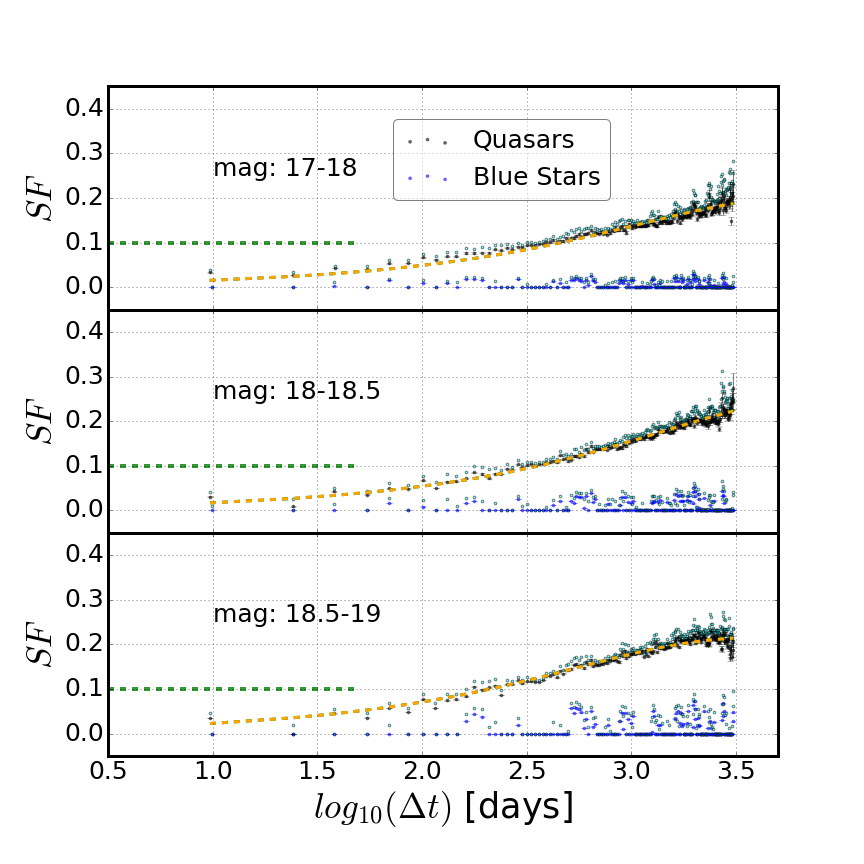
\includegraphics[width=1.15\columnwidth, center]{Fig_4_SF_QSO_starsB_r_cut.png}
 \caption{Three panels depict the impact that applying correction factors f\textsubscript{c} to errors $\sigma(\Delta m)$ has on the structure function for blue stars and quasars in the observer's frame t\textsubscript{obs} (see Fig.~\ref{fig:5} for the same in the quasar restframe, t\textsubscript{rest}). In the middle of each panel we list the SDSS r-magnitude used to select quasars and stars. It is noteworthy that applying the correction factor the apparently discrepant variability of non-variable standard stars  vanishes (the residual SF is consistent with the noise rms of 0.05\textsuperscript{mag}). The variability of quasars also decreases  to a level consistent with noise. Therefore the corrected SF of quasars at short time scales ($\log_{10}(\Delta t) < 1.7$) agrees with a lack of variability, which is consistent with the previous SDSS results (upper limits of 0.1\textsuperscript{mag} marked by green dashed lines) (see \citep{macleod2011}).}
\end{figure}

\begin{figure}
\label{fig:5}
 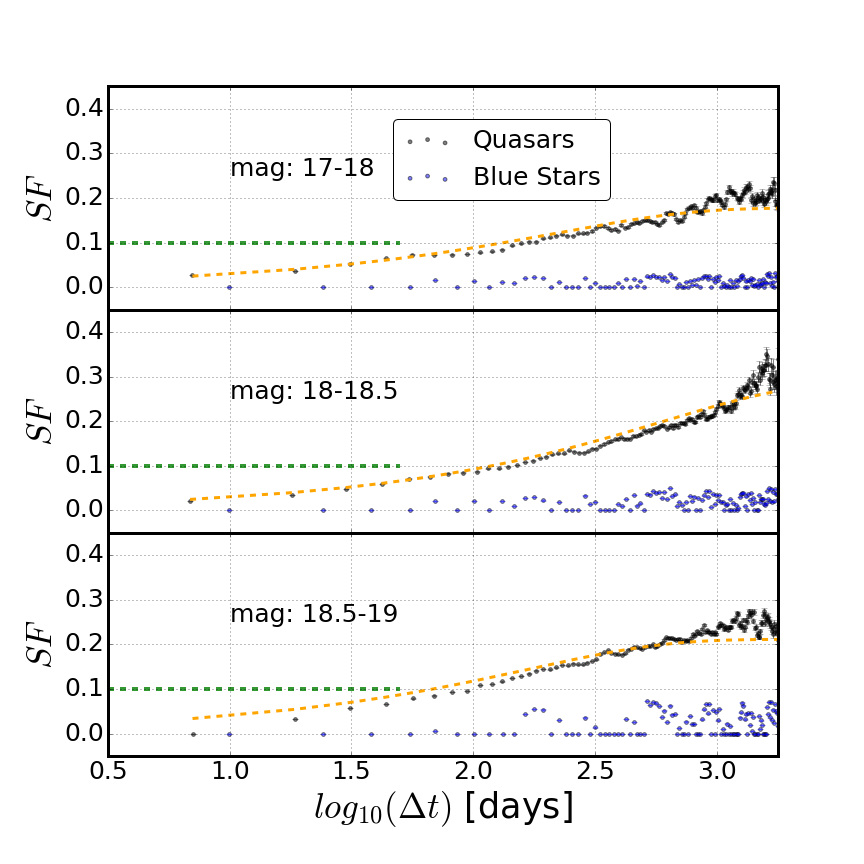
\includegraphics[width=1.15\columnwidth, center]{Fig_5_SF_QSO_starsB_r_cut_rest.png}
 \caption{The same as Fig.~\ref{fig:4}, but plotted in the quasar restframe : t\textsubscript{rest} = t\textsubscript{obs} / (1+z), using known quasar redshifts from SDSS \citep{macleod2010}.   In the middle of each panel we list the SDSS r-magnitude used for selection. The restframe correction shifts time lags to shorter timescales, but does not affect our predictions about the lack of variability in quasars on short timescales ($\log_{10}(\Delta t) < 1.7$).} %The apparent downturn in the $SF$ of quasars, as compared to Fig.4, is due to the smaller number of points in bins of higher $\Delta t$, which leads to smaller bin dispersion in $\Delta m$. }
\end{figure}



\section{PTF Data}

We compare our CRTS results against recently released  PTF Data Release 3 lightcurves \footnote{\url{http://www.ptf.caltech.edu/page/lcdb}}. We queried the NASA/IPAC Infrared Science Archive \footnote{\url{https://irsa.ipac.caltech.edu}} 'PTF Objects' catalog against the list of ra, dec of 7601 spectroscopically confirmed Stripe 82 quasars, and 48250 standard stars (same as obtained from the CRTS database previously).  A positional multi-object search with a matching radius of 2 arcsec , with  a flag 'ngoodobs' > 10,  resulted with  6471 quasars and 38776 stars.  For these objects we obtained time series data from 'PTF Lightcurve Table' catalog.  We select lightcurves corresponding to individual objects by grouping with SDSS ra, because the PTF coordinates might vary from  one CCD chip to another by up to 1.5 arcsec (David Schuppe, priv.comm.)  We avoid grouping by PTF object id ('oid'), because a new detection of the same object on a different chip assigned different 'oid'. For example, there  are 38786 'oid's  and only 38776  unique 'ra'  in the stellar sample, with 10  id's  corresponding to those objects that  have been detected on more than one ccd, in the overlapping region. 

We processed the PTF lightcurves in exactly the same way as the CRTS lightcurves. We first performed day-averaging, using the weighted error as the measure of uncertainty on day-averaged  brightness measurement. We further selected only those objects that have been observed over at least 10 separate days (i.e. have over 10 day-averaged epochs). Only 2753 quasars and 15714 stars, i.e. less than 50\% sources, fulfill these criteria.  For those objects, we enrich the PTF information with the SDSS catalog photometry, and calculate the magnitude vs. time difference ('master') files : $\Delta m_{jk} = m_{j} - m_{k}$, $\Delta t_{jk} = t_{j} - t_{k}$ for $j>k$, with errors  $\sigma(\Delta m_{jk})^{2} = \sigma_{j}^{2} + \sigma_{k}^{2}$. 


\begin{figure}
\label{fig:2a}
 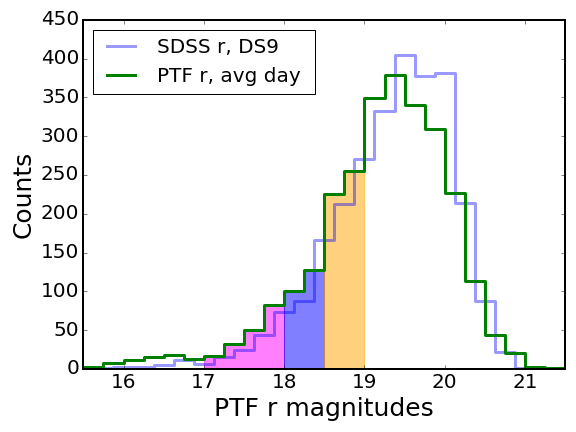
\includegraphics[width=1.15\columnwidth, center]{Fig_2_Quasar_PTF_population_selection.png}
 \caption{Magnitude selection in PTF quasar data. Two histograms represent the magnitude distribution for PTF quasars using either   $\langle m_{i} \rangle $: the mean day-averaged PTF r-band magnitudes, or the SDSS r-band photometry from DS9 catalog. Shaded regions illustrate portion of the population selected in each magnitude bins. It makes sense that the majority of quasars do not end up contributing to the final analysis given that we focus on the best-quality bright-end of the quasar population, which peaks  at around 19\textsuperscript{th} magnitude.   }
\end{figure}


\begin{table}
\centering
\caption{Analoguously to ~\ref{tab:object_count}, the count of stars and quasars, selected by their SDSS r-magnitude from PTF data (see Fig.~\ref{fig:2a}). For all objects we also required that the PTF lightcurve error is smaller than 0.3\textsuperscript{mag}.}
\label{tab:object_count_PTF}
\begin{tabular}{ l|ccc } 
% \hline
r-mag  & red stars & blue stars & quasars \\ 
 \hline
17-18   & 1243 & 1077   & 90    \\ 
18-18.5 & 825 &  497  & 160   \\ 
18.5-19 & 913 &  548  & 377   
% \hline
\end{tabular}
\end{table}

To plot structure functions we selected quasars, blue and red stars according to their SDSS r-magnitude, and PTF average lightcurve error (see Table ~\ref{tab:object_count_PTF}). In each magnitude bin,  for a given type of object we thus have over 100 000 magnitude-difference points  (for quasars averaging across magnitude bins, $N_{\Delta m} = 117 694 $, while for blue and red stars, it is 364 606 and 555 668, respectively ). We removed the outliers in $\Delta {m_{ij}}$ stemming from the photometric measurement outliers (we did not perform any sigma clipping on the input lightcurves). Requiring $|\Delta m | < 1.0$ we discarded less than 2\% of $\Delta m$ points. Similar to the CRTS data, we split the magnitude-binned samples into  200 linearly spaced bins in $\Delta t $ space. For each bin we  calculated the  structure function  ($\sigma_{0}$) , mean ($\mu_{0}$),  interquartile range robust standard deviation ($\sigma_{G}$), and the standard deviation ($\sigma_{st.dev.}$), as described in Sec.~\ref{sec:analysis}. We find that regardless of the magnitude bin,  PTF quasars do not exhibit signs of variability at $\log_{10}{(\Delta t)} < 	2.0$, i.e. $\Delta t$< 100 days.  Unlike CRTS, for PTF both stars and quasars the SF $\approx$ 0 at these short timescales (see Fig.~\ref{fig:2_PTF}). 


\begin{figure}
\label{fig:2_PTF}
 \includegraphics[width=1.15\columnwidth, center]{{Fig_2_18.5-19.0_PTF_panels}.png}
 \caption{The statistics for the subsample of 377 PTF quasars (black points), 548 "blue" stars (blue points), and 913 "red" stars (red points), all  chosen according to the SDSS r magnitude $18.5 < \mathrm{m} < 19$. Red and blue stars have  $1 < \mathrm{g-i} < 3$ and  $-1 < \mathrm{g-i} < 1$ respectively. All pairwise brightness differences  in PTF r-band are binned in $200$ linearly spaced bins of $\Delta t$. For each bin, we calculate different statistics, from top to bottom panels: the standard deviation $\sigma_{stdev}$, the robust Gaussian deviation based on the interquartile range $\sigma_{G}$, the structure function $SF$, and  the mean value of $\Delta m$  per bin: $\mu$. Both $\mu$ and $\sigma$ are found from the 2D maximum of the log-likelihood $L_{p}$ on the $[\mu,\sigma]$ grid (see eq.~\ref{eq:logP}, and \citep{ivezic2014}).  Yellow dashed line on the third panel traces the fiducial Damped Random Walk model. For these uncorrected PTF data, it is evident that there is no sign of variability for quasars on short timescales ($\Delta t < 100 \, \mathrm{days}$), unlike for CRTS data (see Fig.~\ref{fig:2}). Standard stars are used as a good quality comparison, and as expected, they have no variability ($SF \approx 0$). However,  the mean does not stay as close to 0 as for CRTS data - note an asymmetric dip around $\log_{10} (\Delta t) \approx 2.7$ that signifies some issues with the data pipeline. This shaded region in $\mu$ space is further explored on Fig.~\ref{fig:2_PTF_hist}.}
 
\end{figure}


\begin{figure}
\label{fig:2_PTF_hist}
 \includegraphics[width=1.15\columnwidth, center]{{Fig_2_18.5-19.0_log_2.6-2.75_hist}.png}
 \caption{Normalized histograms for $\Delta m_{ij}$ from the shaded region on the bottom panel of Fig.~\ref{fig:2_PTF}. Red, blue and black solid lines correspond to red stars, blue stars, and quasars, respectively. Vertical dashed lines outline the mean $\Delta m_{ij}$ for each population. In each case, the mean is below 0. }
 % anything more here  ? }
\end{figure}

\section{Conclusions}
We analyzed the error properties of the CRTS sample of quasars and standard stars.  We find that the errors require correction on the order of 20\%, and that without this correction even non-variable standard stars show structure function variability on the level of 0.1\textsuperscript{mag}. Through analysis of $\chi$ distribution we show that the listed errors are under- or overestimated.  

\section*{Acknowledgements}

We thank Eric Bellm for all help with data retrieval and reduction of PTF lightcurves .  

We thank Neven Caplar for  fruitful discussions on the use of PTF data and structure function methodology. 

Funding for the SDSS and SDSS-II has been provided by the Alfred P. Sloan Foundation, the Participating Institutions, the National Science Foundation, the U.S. Department of Energy, the National Aeronautics and Space Administration, the Japanese Monbukagakusho, the Max Planck Society, and the Higher Education Funding Council for England. The SDSS Web Site is http://www.sdss.org/.

The SDSS is managed by the Astrophysical Research Consortium for the Participating Institutions. The Participating Institutions are the American Museum of Natural History, Astrophysical Institute Potsdam, University of Basel, University of Cambridge, Case Western Reserve University, University of Chicago, Drexel University, Fermilab, the Institute for Advanced Study, the Japan Participation Group, Johns Hopkins University, the Joint Institute for Nuclear Astrophysics, the Kavli Institute for Particle Astrophysics and Cosmology, the Korean Scientist Group, the Chinese Academy of Sciences (LAMOST), Los Alamos National Laboratory, the Max-Planck-Institute for Astronomy (MPIA), the Max-Planck-Institute for Astrophysics (MPA), New Mexico State University, Ohio State University, University of Pittsburgh, University of Portsmouth, Princeton University, the United States Naval Observatory, and the University of Washington. 


\section*{Appendix A}
  %- derivation of how fc impacts an individual error measurement
In Sec.~\ref{sec:results} we show how $f_{c}$ corrects the value of the magnitude-difference error : $\sigma(\Delta m_{j,k})$. Now since $\sigma(m_{j}) = 1 / \sqrt{\sum{w_{j}}}$, and $w_{j} = 1 / e_{j}^{2}$; if we assume that errors are homoscedastic, i.e. $e_{j} = e$, then $\sigma(m) = e / \sqrt{M}$, where $M$ is the number of intra-night observations.  
So since we require $\sigma(\Delta m)_{corr} = f_{c} \, \sigma(\Delta m)$, we have $e_{corr} = f_{c} e$,  so that $f_{c}$ applies as a multiplicative correction factor both for weight-based day-averaged magnitude errors, as well as the raw errors. 




%%%%%%%%%%%%%%%%%%%%%%%%%%%%%%%%%%%%%%%%%%%%%%%%%%

%%%%%%%%%%%%%%%%%%%% REFERENCES %%%%%%%%%%%%%%%%%%

% The best way to enter references is to use BibTeX:
\bibliographystyle{apj}
%\bibliographystyle{mnras}
\bibliography{references} % if your bibtex file is called example.bib

%%%%%%%%%%%%%%%%%%%%%%%%%%%%%%%%%%%%%%%%%%%%%%%%%%


% Don't change these lines
\bsp	% typesetting comment
\label{lastpage}
\end{document}

% End of mnras_template.tex
